%!TEX root = ../effc_top.tex

\begin{frame}{Operations at odd primes}

	\pause

	Steenrod squares come from making a \textbf{binary} coproduct $C \to C^{\ot 2}$ cocommutative up to coherent homotopies.

	\medskip\pause

	Steenrod also defined operations (for $\beta \in \{0,1\}$)
	\[
	\beta^{\varepsilon} P_k \colon H^\bullet(X; \Fp) \to H^\bullet(X; \Fp).
	\]

	\pause

	They come from making a coproduct $C \to C^{\ot p}$ cocommutative up to coherent homotopies.

	\medskip\pause

	A coherent structure controlling these is that of an $E_\infty$-coalgebra.

	\medskip\pause

	$E_\infty$-structures have a long history:
	\begin{itemize}
		\item (co)homology operations,
		\item recognition of infinite loop spaces,
		\item algebraic models of the homotopy category.
	\end{itemize}
\end{frame}

\begin{frame}{An $E_\infty$-coalgebra on chains} \pause
	\begin{theorem}[Med.]
		The collection of maps $\gchains(\gsimplex^n) \to \gchains(\gsimplex^n)^{\otimes r}$ obtained from compositions of
		\begin{align*}
			\Delta &\colon \gchains(\gsimplex^n) \to \gchains(\gsimplex^n)^{\otimes 2}
			\qquad \text{(AW diagonal)} \\
			\ast &\colon \gchains(\gsimplex^n)^{\otimes 2} \to \gchains(\gsimplex^n)
			\qquad \text{(Join map)}
		\end{align*}
		defines an $E_\infty$-coalgebra on simplicial chains.
	\end{theorem}

	\pause

	\qquad \qquad \scalebox{0.7}{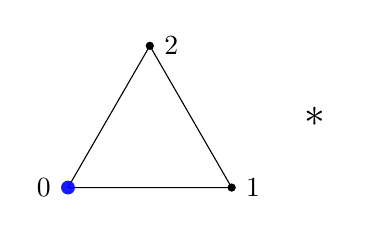
\begin{tikzpicture}[scale=.6]
\coordinate (A) at (210:2);
\coordinate (B) at (-30:2);
\coordinate (C) at (90:2);

\draw[draw=black] (A) -- (B) -- (C) -- (A);

\node[circle,fill=blue, opacity=.9, inner sep=0pt,minimum size=5pt, label=left:{0}] (a) at (A) {};
\node[circle,fill=black,inner sep=0pt,minimum size=3pt, label=right:{$1$}] (a) at (B) {};
\node[circle,fill=black,inner sep=0pt,minimum size=3pt, label=right:{$2$}] (a) at (C) {};

\node[scale=1.5] at (3.5,0.5) {$\ast$};
\end{tikzpicture}
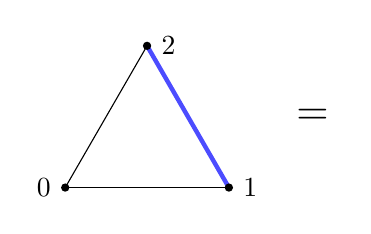
\begin{tikzpicture}[scale=.6]
\coordinate (A) at (210:2);
\coordinate (B) at (-30:2);
\coordinate (C) at (90:2);

\draw[draw=blue,  ultra thick, draw opacity=.7] (B) -- (C);
\draw[draw=black] (C) -- (A);
\draw[draw=black] (A) -- (B);

\node[circle,fill=black,inner sep=0pt,minimum size=3pt, label=left:{$0$}] (a) at (A) {};
\node[circle,fill=black,inner sep=0pt,minimum size=3pt, label=right:{$1$}] (a) at (B) {};
\node[circle,fill=black,inner sep=0pt,minimum size=3pt, label=right:{$2$}] (a) at (C) {};

\node[scale=1.5] at (3.5,.5) {=};
\end{tikzpicture}
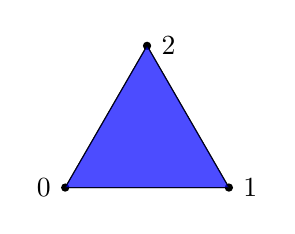
\begin{tikzpicture}[scale=.6]
\coordinate (A) at (210:2);
\coordinate (B) at (-30:2);
\coordinate (C) at (90:2);

\draw[draw=black] (A) -- (B) -- (C) -- (A);

\node[circle,fill=black,inner sep=0pt,minimum size=3pt, label=left:{$0$}] (a) at (A) {};
\node[circle,fill=black,inner sep=0pt,minimum size=3pt, label=right:{$1$}] (a) at (B) {};
\node[circle,fill=black,inner sep=0pt,minimum size=3pt, label=right:{$2$}] (a) at (C) {};

\draw[draw, fill=blue, opacity=.7] (A) -- (B) -- (C) -- (A);
\end{tikzpicture}}

	\medskip\pause

	Also, versions for: \par
		\qquad \textcolor{pblue}{cubical} (Kaufmann--Med.) and \par
		\qquad \textcolor{pblue}{multisimplicial} (Med.--Pizzi--Salvatore) chains.
\end{frame}

\begin{frame}[fragile]{May--Steenrod structures}

	\vskip-5pt\pause

	\begin{block}{Construction (Kaufmann-Med.)}
		Explicit cup-$(p,i)$ coproducts defining \textcolor{pblue}{operations} on $H^\bullet(-; \Fp)$.
	\end{block}

	\pause

	\begin{block}{Implementation (Med.)}
		In the computer algebra system \textcolor{pblue}{\texttt{ComCH}}.
	\end{block}

	\pause

	For example, $\Delta_{3,2}[0,1,2]$ is equal to

	\begin{verbatim}
		- [0,1][0,1,2][0,1] + [0,1,2][0,2][0,1] + [0,2][0,2][0,1,2]
		- [0,1,2][0,1,2][1] - [0,2][0,1,2][1,2] + [0,1,2][1,2][1,2]
		- [0,1][1,2][0,1,2] - [0,1,2][2][0,1,2] - [0][0,1,2][0,1,2]
	\end{verbatim}

	\pause

	\textcolor{pblue}{Future directions:} (from the even to odd primes)

	\pause
	\begin{enumerate}
		\item Faster implementations for use in TDA. \pause \\
		\item Relation to higher category theory. \pause \\
		\item Connections to convex geometry. \pause \\
		\item Cartan and Adem coboundaries. \pause \\
		\item Where are these used in physics?
	\end{enumerate}
\end{frame}